\chapter{Requisits del sistema}
\usetikzlibrary{positioning, shadows}
\label{chap:requisits}

Abans d'iniciar el desenvolupament de l'aplicació d'escriptori NUMEN, s'ha dut a terme una anàlisi detallada de requisits, seguint una metodologia rigorosa per garantir l'èxit del projecte. Aquesta fase ha estat clau per identificar les funcionalitats necessàries, establir les característiques tècniques que ha de complir el sistema i definir-ne l'abast, assegurant que la solució final satisfaci les necessitats de l'usuari expert, tant en l'àmbit del càlcul numerològic complex com en la interpretació assistida per Intel·ligència Artificial.

Els requisits s'han classificat en funcionals, no funcionals i de domini, codificant-los per facilitar-ne la traçabilitat i assignant-los una prioritat (alta, mitjana o baixa) en funció de la seva importància per al correcte funcionament del sistema. A més, per facilitar l'anàlisi de dependències i la planificació del desenvolupament, s'han agrupat en blocs lògics.

Tot seguit, es presenta un glossari amb els termes principals utilitzats al llarg d'aquest capítol, per garantir-ne la claredat i coherència terminològica.

\section{Glossari de Termes}

\begin{description}
    \item[App Web / Escriptori] Aplicació híbrida desenvolupada en Flutter. Funciona principalment com a aplicació web accessible des de qualsevol navegador, però conserva la capacitat de compilar-se com a executables d'escriptori (Windows) per a ús \textit{offline} si és necessari.
    \item[Servei IA] Part del sistema que gestiona la comunicació amb Google Gemini (LLM) per generar les interpretacions textuals.
    \item[Usuari] Persona que utilitza el sistema per realitzar estudis numerològics.
    \item[Administrador] Persona encarregada del manteniment tècnic i l'ajust dels *prompts*.
    \item[Figura Espiritual] Representació gràfica dinàmica de l'Home de Vitruvi, construïda visualment via manipulació de vectors SVG en funció de les dades de l'usuari.
    \item[Nombres Kàrmics] Nombres específics (13, 14, 16, 19) que indiquen lliçons pendents, o en el context de la Inclusió, les cases buides (sense habitants).
    \item[Inclusió] Esquema numerològic organitzat en 9 "Cases" o àrees de la vida.
    \item[Prompt] Instrucció textual estructurada que s'envia a l'IA.
\end{description}

\section{Esquema del Sistema}

El sistema NUMEN compta amb dos actors principals:
\begin{itemize}
    \item \textbf{Usuari:} Introdueix dades i consumeix els informes.
    \item \textbf{Administrador:} Gestiona la infraestructura i qualitat de la IA.
\end{itemize}

\begin{figure}[h]
    \centering
    \begin{tikzpicture}[node distance=2.5cm, auto,
        actor/.style={circle, draw, minimum size=1cm, inner sep=0pt, fill=gray!10},
        block/.style={rectangle, draw, rounded corners, minimum width=2.5cm, minimum height=1.5cm, fill=blue!10, align=center},
        cloudNode/.style={cloud, draw, cloud puffs=10, cloud puff arc=120, aspect=2, minimum width=3cm, fill=green!10, align=center},
        line/.style={draw, -latex', thick}]

        % Nodes
        \node [actor] (user) {Usuari};
        \node [block, right of=user, node distance=4cm] (app) {App\\(Càlcul Local)};
        \node [block, right of=app, node distance=4cm] (ai) {Servei IA\\(API)};
        \node [cloudNode, below of=ai, node distance=3cm] (db) {Base de Dades\\(FireBase)};
        \node [actor, left of=db, node distance=4cm] (admin) {Admin};

        % Edges
        % Edges
        \path [line] (user) to[bend left=25] node[above] {Input / Feedback} (app);
        \path [line] (app) to[bend left=15] node[below] {Resultats} (user);
        \path [line] (app) to[bend left=15] node[above] {Prompt} (ai);
        \path [line] (ai) to[bend left=30] node[below] {Interpretació} (app);
        \path [line] (ai) -- node[right] {Dades Entrenament} (db);
        \path [line] (admin) -- node[above] {Gestió} (db);
        \path [line] (admin) -- node[left] {Manteniment} (app);

    \end{tikzpicture}
    \caption{Esquema d'alt nivell del sistema NUMEN.}
    \label{fig:esquema_sistema}
\end{figure}

\section{Requeriments del Sistema}

\subsection{Requeriments Funcionals}

\begin{table}[H]
    \centering
    \begin{tabular}{|l|l|l|p{8cm}|}
    \hline
    \textbf{ID} & \textbf{Prioritat} & \textbf{Actor} & \textbf{Descripció} \\ \hline
    RF1 & Alta & Usuari & El sistema ha de permetre introduir la data de naixement i nom complet. \\ \hline
    RF2 & Alta & Sistema & Execució automàtica dels algorismes de càlcul (Gematria, Cicles, NL). \\ \hline
    RF3 & Alta & Sistema & Visualització de resultats en graelles i llistes. \\ \hline
    RF4 & Alta & Sistema & Generació dinàmica de l'Home de Vitruvi (SVG) segons dades. \\ \hline
    RF5 & Alta & Sistema & Detecció i marcatge visual de Karmes i Nombres Mestres. \\ \hline
    RF6 & Alta & Usuari & L'usuari ha de poder sol·licitar una interpretació a la IA. \\ \hline
    RF7 & Alta & Sistema & Mostratge de la interpretació en format text natural estructurat. \\ \hline
    RF8 & Mitja & Usuari & L'usuari ha de poder valorar la resposta i afegir comentaris qualitatius (Feedback). \\ \hline
    RF9 & Alta & Sistema & Emmagatzematge persistent de consultes i feedback (Firestore). \\ \hline
    RF10 & Alta & Sistema & Generació d'informe en **PDF Natiu** (Vectorial) descarregable. \\ \hline
    RF13 & Alta & Sistema & Generació d'un ``Enllaç Compartit'' amb caducitat de 24h. \\ \hline
    RF14 & Alta & Sistema & Adaptació de la interfície a dispositius mòbils (**Responsive Design**). \\ \hline
    \end{tabular}

    \caption{Requisits funcionals del sistema.}
    \label{tab:req_funcionals}
\end{table}

\subsection{Matriu de dependències entre requisits funcionals}

\begin{table}[H]
    \centering
    \resizebox{\textwidth}{!}{%
    \begin{tabular}{|l|c|c|c|c|c|c|c|c|c|c|c|c|c|c|}
    \hline
         & \textbf{RF1} & \textbf{RF2} & \textbf{RF3} & \textbf{RF4} & \textbf{RF5} & \textbf{RF6} & \textbf{RF7} & \textbf{RF8} & \textbf{RF9} & \textbf{RF10} & \textbf{RF11} & \textbf{RF12} & \textbf{RF13} & \textbf{RF14} \\ \hline
    \textbf{RF1} & & X & & & & & & & & & & & & \\ \hline
    \textbf{RF2} & & & X & X & X & X & & & & X & & & & \\ \hline
    \textbf{RF3} & & & & & & & & & & X & & & X & \\ \hline
    \textbf{RF4} & & & & & & & & & & X & & & & \\ \hline
    \textbf{RF5} & & & & & & & & & & X & & & & \\ \hline
    \textbf{RF6} & & & & & & & X & & X & & & & & \\ \hline
    \textbf{RF7} & & & & & & & & X & X & X & & & X & \\ \hline
    \textbf{RF8} & & & & & & & & & X & & & & & \\ \hline
    \textbf{RF9} & & & & & & & & & & & X & & & \\ \hline
    \textbf{RF10}& & & & & & & & & & & & & X & \\ \hline
    \textbf{RF11}& & & & & & & & & & & & X & & \\ \hline
    \textbf{RF12}& & & & & & & & & & & & & & \\ \hline
    \textbf{RF13}& & & & & & & & & & & & & & \\ \hline
    \textbf{RF14}& & & & & & & & & & & & & & \\ \hline
    \end{tabular}%
    }
    \caption{Matriu de dependències entre requisits funcionals.}
    \label{tab:dependencies_func}
\end{table}

\subsection{Requeriments No Funcionals}

\begin{table}[H]
    \centering
    \begin{tabular}{|l|l|p{5cm}|p{5cm}|}
    \hline
    \textbf{ID} & \textbf{Prioritat} & \textbf{Descripció} & \textbf{Verificació} \\ \hline
    RNF1 & Alta & Usabilitat intuïtiva (Mobile First). & Test d'usuari sense formació prèvia. \\ \hline
    RNF2 & Mitja & Latència IA < 10s. & Mesura en xarxa 4G/Fibra. \\ \hline
    RNF3 & Alta & Compatibilitat Web i Escriptori (Windows). & Execució en Chrome, Edge i .exe natiu. \\ \hline
    RNF4 & Alta & Seguretat de les dades (Regles Firestore). & Intent d'accés no autoritzat bloquejat. \\ \hline
    RNF5 & Alta & Qualitat d'impressió professional. & PDF vectorial escalable sense pixelat. \\ \hline
    \end{tabular}
    \caption{Requisits no funcionals del sistema.}
    \label{tab:req_nofuncionals}
\end{table}

\subsection{Requeriments del Domini}

\begin{table}[H]
    \centering
    \begin{tabular}{|l|l|p{10cm}|}
    \hline
    \textbf{ID} & \textbf{Prioritat} & \textbf{Descripció} \\ \hline
    RD1 & Alta & Càlculs estrictes segons Mètode Coquatrix. \\ \hline
    RD2 & Alta & To de la IA: Empàtic, constructiu i respectuós. \\ \hline
    RD3 & Mitja & Privacitat: Anonimització de dades sensibles en logs. \\ \hline
    RD4 & Alta & Tractament correcte de Nombres Mestres (11, 22, 33). \\ \hline
    \end{tabular}
    \caption{Requisits del domini.}
    \label{tab:req_domini}
\end{table}

\section{Matriu de dependències entre tots els requisits}

\begin{table}[H]
    \centering
    \resizebox{\textwidth}{!}{%
    \begin{tabular}{|l|c|c|c|c|c|c|c|c|c|c|c|c|c|c|c|c|c|c|c|c|c|c|c|c|}
    \hline
         & \textbf{RF1} & \textbf{RF2} & \textbf{RF3} & \textbf{RF4} & \textbf{RF5} & \textbf{RF6} & \textbf{RF7} & \textbf{RF8} & \textbf{RF9} & \textbf{RF10} & \textbf{RF11} & \textbf{RF12} & \textbf{RF13} & \textbf{RF14} & \textbf{RNF1} & \textbf{RNF2} & \textbf{RNF3} & \textbf{RNF4} & \textbf{RNF5} & \textbf{RD1} & \textbf{RD2} & \textbf{RD3} & \textbf{RD4} & \textbf{RD5} \\ \hline
    \textbf{RF1} & & X & & & & & & & & & & & & & & & & & & & & & & \\ \hline
    \textbf{RF2} & & & X & X & X & X & & & & X & & & & & & & & X & & & X & \\ \hline
    \textbf{RF3} & & & & & & & & & & X & & & X & & X & & & & & & & & & \\ \hline
    \textbf{RF4} & & & & & & & & & & X & & & & & & & & & & & & & & X \\ \hline
    \textbf{RF5} & & & & & & & & & & X & & & & & & & & & & & & & & \\ \hline
    \textbf{RF6} & & & & & & & X & & X & & & & & & & X & & & & & & & & \\ \hline
    \textbf{RF7} & & & & & & & & X & X & X & & & X & & X & & & & & & X & & & \\ \hline
    \textbf{RF8} & & & & & & & & & X & & & & & & & & & & & & & & & \\ \hline
    \textbf{RF9} & & & & & & & & & & & X & & & & & & X & & & & X & & & \\ \hline
    \textbf{RF10}& & & & & & & & & & & & & X & & & & & X & & & & & & \\ \hline
    \end{tabular}%
    }
    \caption{Matriu de dependències global.}
    \label{tab:dependencies_global}
\end{table}



\section{Relació amb la Planificació (Mapatge de Requisits)}

La Figura \ref{fig:mapa_requisits} il·lustra com els requisits s'implementen a través dels Paquets de Treball (PT) definits al Capítol 4.

\begin{figure}[H]
    \centering
    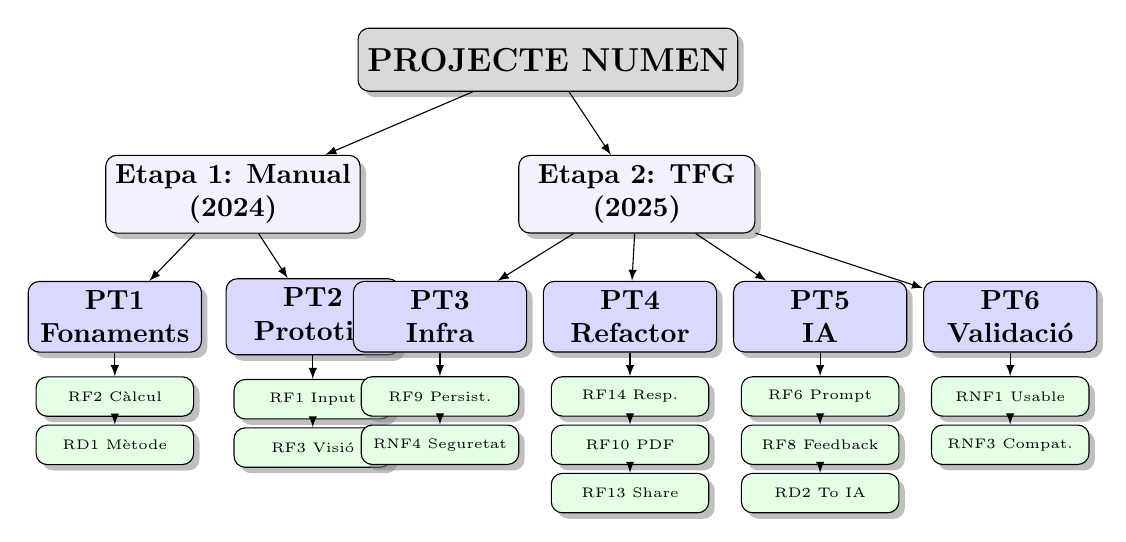
\begin{tikzpicture}[
        node distance=0.5cm and 0.2cm,
        every node/.style={draw, rounded corners, align=center, font=\scriptsize, fill=white, drop shadow},
        root/.style={fill=gray!30, font=\large\bfseries, minimum width=3cm, minimum height=0.8cm},
        etapa/.style={fill=blue!5, font=\bfseries, minimum width=3cm, minimum height=0.7cm},
        pt/.style={fill=blue!15, font=\bfseries, minimum width=2.2cm, minimum height=0.7cm},
        req/.style={fill=green!10, font=\tiny, minimum width=2cm, minimum height=0.5cm},
        link/.style={-latex, thin}
    ]

    % Root
    \node[root] (root) {PROJECTE NUMEN};

    % Level 1: Stages
    \node[etapa, below=0.8cm of root, xshift=-4cm] (etapa1) {Etapa 1: Manual\\(2024)};
    \node[etapa, right=2cm of etapa1] (etapa2) {Etapa 2: TFG\\(2025)};

    \draw[link] (root) -- (etapa1);
    \draw[link] (root) -- (etapa2);

    % Level 2: PTs
    % Etapa 1 PTs
    \node[pt, below=0.6cm of etapa1, xshift=-1.5cm] (pt1) {PT1\\Fonaments};
    \node[pt, right=0.3cm of pt1] (pt2) {PT2\\Prototip};
    \draw[link] (etapa1) -- (pt1);
    \draw[link] (etapa1) -- (pt2);

    % Etapa 2 PTs
    \node[pt, below=0.6cm of etapa2, xshift=-2.5cm] (pt3) {PT3\\Infra};
    \node[pt, right=0.2cm of pt3] (pt4) {PT4\\Refactor};
    \node[pt, right=0.2cm of pt4] (pt5) {PT5\\IA};
    \node[pt, right=0.2cm of pt5] (pt6) {PT6\\Validació};
    \draw[link] (etapa2) -- (pt3);
    \draw[link] (etapa2) -- (pt4);
    \draw[link] (etapa2) -- (pt5);
    \draw[link] (etapa2) -- (pt6);

    % Level 3: Requirements mapping
    % PT1 (Fonaments) -> RF2 (Algorismes), RD1 (Mètode)
    \node[req, below=0.3cm of pt1] (rf2) {RF2 Càlcul};
    \node[req, below=0.1cm of rf2] (rd1) {RD1 Mètode};
    \draw[link] (pt1) -- (rf2);
    \draw[link] (rf2) -- (rd1);

    % PT2 (Prototip) -> RF1 (Input), RF3 (Llistes)
    \node[req, below=0.3cm of pt2] (rf1) {RF1 Input};
    \node[req, below=0.1cm of rf1] (rf3) {RF3 Visió};
    \draw[link] (pt2) -- (rf1);
    \draw[link] (rf1) -- (rf3);

    % PT3 (Infra) -> RF9 (DB), Cloud
    \node[req, below=0.3cm of pt3] (rf9) {RF9 Persist.};
    \node[req, below=0.1cm of rf9] (rnf4) {RNF4 Seguretat};
    \draw[link] (pt3) -- (rf9);
    \draw[link] (rf9) -- (rnf4);

    % PT4 (Refactor) -> RF10 (PDF), RF13 (Share), RF14 (Resp)
    \node[req, below=0.3cm of pt4] (rf14) {RF14 Resp.};
    \node[req, below=0.1cm of rf14] (rf10) {RF10 PDF};
    \node[req, below=0.1cm of rf10] (rf13) {RF13 Share};
    \draw[link] (pt4) -- (rf14);
    \draw[link] (rf14) -- (rf10);
    \draw[link] (rf10) -- (rf13);

    % PT5 (IA) -> RF6, RF7, RF8, RD2
    \node[req, below=0.3cm of pt5] (rf6) {RF6 Prompt};
    \node[req, below=0.1cm of rf6] (rf8) {RF8 Feedback};
    \node[req, below=0.1cm of rf8] (rd2) {RD2 To IA};
    \draw[link] (pt5) -- (rf6);
    \draw[link] (rf6) -- (rf8);
    \draw[link] (rf8) -- (rd2);

    % PT6 (Validació) -> RNF1, RNF3
    \node[req, below=0.3cm of pt6] (rnf1) {RNF1 Usable};
    \node[req, below=0.1cm of rnf1] (rnf3) {RNF3 Compat.};
    \draw[link] (pt6) -- (rnf1);
    \draw[link] (rnf1) -- (rnf3);

    \end{tikzpicture}
    \caption{Traçabilitat entre Paquets de Treball i Requisits.}
    \label{fig:mapa_requisits}
\end{figure}
